\documentclass{article}
\usepackage{tikz}
\usetikzlibrary{arrows.meta}

\begin{document}

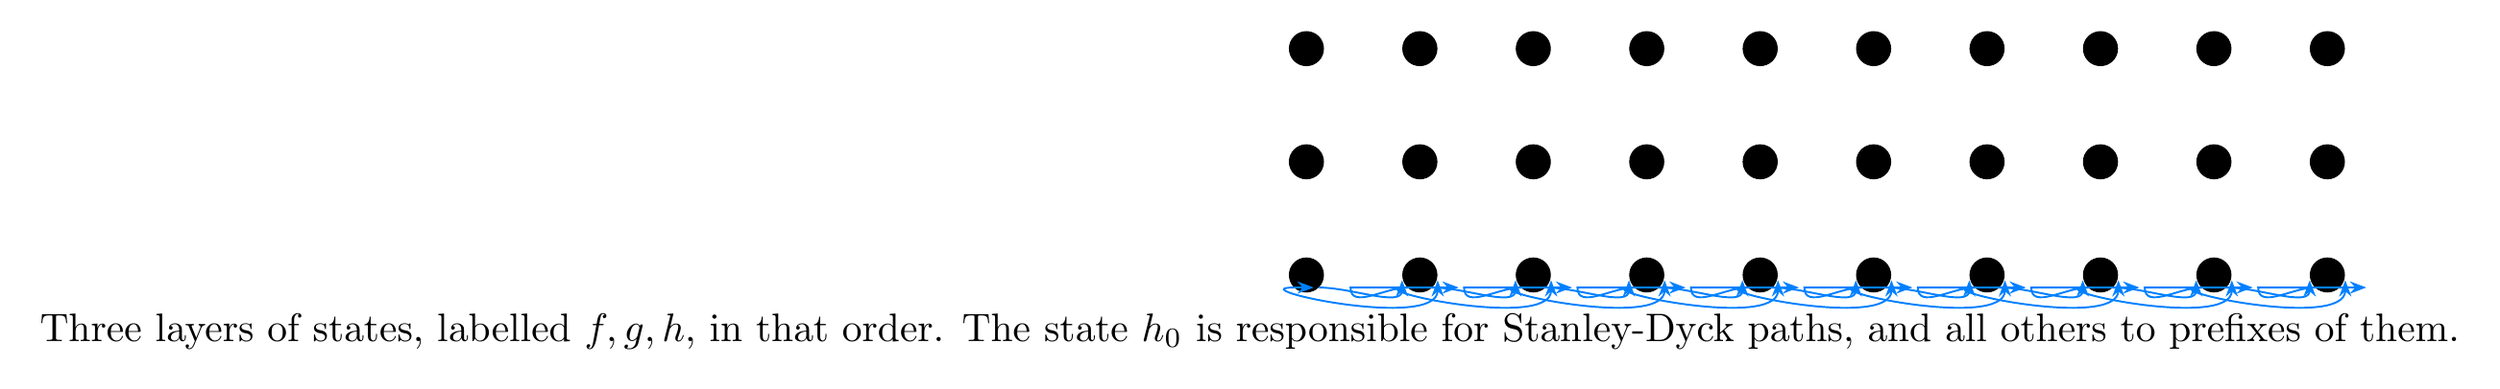
\begin{tikzpicture}[scale=1.5, every node/.style={transform shape}, shorten >=2pt]
    % Define colors
    \definecolor{stateColor}{RGB}{0,0,0}
    \definecolor{transitionColor}{RGB}{0,128,255}

    % Define nodes
    \tikzset{
        state/.style = {
            circle,
            draw,
            fill = stateColor,
            inner sep = 0pt,
            minimum size = 3mm
        },
        transition/.style = {
            draw,
            -Stealth,
            line width = 0.7pt,
            color = transitionColor
        }
    }

    % Draw states
    \foreach \x in {0,...,9} {
        \node[state] (s\x) at (\x, 0) {};
        \node[state] (s\x') at (\x, 1) {};
        \node[state] (s\x'') at (\x, 2) {};
    }

    % Draw edges between states
    \foreach \x [evaluate=\x as \prevx using int(\x-1)] in {1,...,9} {
        \draw[transition] (s\prevx.south east) to[out=0,in=-90] (s\x.west);
        \draw[transition] (s\prevx.south west) to[out=180,in=-90] (s\x.east);
    }

    % Draw horizontal lines
    \draw[transition] (s0.south west) -- (s0.south east);
    \draw[transition] (s1.south west) to[out=180,in=-90] ++(-0.5,0) -- ++(1,0);
    \draw[transition] (s2.south west) to[out=180,in=-90] ++(-0.5,0) -- ++(1,0);
    \draw[transition] (s3.south west) to[out=180,in=-90] ++(-0.5,0) -- ++(1,0);
    \draw[transition] (s4.south west) to[out=180,in=-90] ++(-0.5,0) -- ++(1,0);
    \draw[transition] (s5.south west) to[out=180,in=-90] ++(-0.5,0) -- ++(1,0);
    \draw[transition] (s6.south west) to[out=180,in=-90] ++(-0.5,0) -- ++(1,0);
    \draw[transition] (s7.south west) to[out=180,in=-90] ++(-0.5,0) -- ++(1,0);
    \draw[transition] (s8.south west) to[out=180,in=-90] ++(-0.5,0) -- ++(1,0);
    \draw[transition] (s9.south west) to[out=180,in=-90] ++(-0.5,0) -- ++(1,0);

    % Add labels
    \foreach \x in {0,...,9} {
        \node at (s\x) {$\bullet$};
        \node at (s\x') {$\bullet$};
        \node at (s\x'') {$\bullet$};
    }

    % Add text below the diagram
    \node at (-0.5, -0.5) {Three layers of states, labelled \( f, g, h \), in that order. The state \( h_{0} \) is responsible for Stanley-Dyck paths, and all others to prefixes of them.};
\end{tikzpicture}

\end{document}